\section{Non-Periodic Sources}
Some of the sources are non deterministic and are given by a Poisson distribution with parameter $\lambda$. To be ablo to create a deterministic model for them a token bucket filter is used. The main parameters are the queue length, $L$, the number of tokens that can be stored, $M$, and the token rate, $r_\mathrm{t}$. A diagram of the filter including the parameters can be seen in \autoref{fig:tokenFilter}.
%
\begin{figure}[H]
	\includegraphics[width = .45\textwidth]{tokenFilter}
	\caption{Diagram of the token bucket filter, including the parameters.}
	\label{fig:tokenFilter}
\end{figure}
%
Once the parameters are known, an affine curve can be used to describe an upper bound for the arrival model similarly as in the case of periodic sources
\begin{flalign}
 \alpha (t) &= M\ P + P\ r_\mathrm{t}\ t 
\end{flalign}
where the burst is given by the maximum number of packets that can pass through if the bucket starts full of tokens.
 
\subsection{Multimedia System}
The parameters for the token bucket are selected looking at the simulation in True Time and finding a value that gives a good result in the number of packets in the queue and in the waiting time. In the case of the multimedia system the parameters are: $L=5$ packets, $M=6$ tokens and $r_\mathrm{t}=50$ tokens per second.

The affine arrival model for the multimedia system is given by
\begin{flalign}
\alpha_\mathrm{multimedia} (t) &= M P_\mathrm{multimedia}+ P_\mathrm{multimedia}\ r_\mathrm{t}\  t  \\
\alpha_\mathrm{multimedia} (t) &= 6 \cdot 11200  + 50 \cdot 11200 t = 67200+560000 t
\end{flalign}
where $P_\mathrm{multimedia}=1400 \cdot 8=11200$ is the packet size in bits.

\subsection{Rear Camera (RC)}
In the case of the rear camera the parameters are: $L=8$ packets, $M=8$ tokens and $r_\mathrm{t}=58$ tokens per second.

The affine arrival model for the multimedia system is given by
\begin{flalign}
\alpha_\mathrm{multimedia} (t) &= M P_\mathrm{RC}+ P_\mathrm{RC}\ r_\mathrm{t}\  t  \\
\alpha_\mathrm{multimedia} (t) &= 8 \cdot 11200  + 58 \cdot 11200 t = 89600+649600 t
\end{flalign}
where $P_\mathrm{RC}=1400 \cdot 8=11200$ is the packet size in bits.

\section{Maximum Backlogs and Waiting Times of the Non-Periodic Sources}
The models for the non-periodic sources and the service curve for the CAN bus can be plotted using RTC. 
\begin{figure}[H]
	\captionbox
	{
		Arrival curves for the Multimedia and service curve for the CAN-bus.
		\label{fig:ArrivalCurvesMultimedia}
	}
	{
		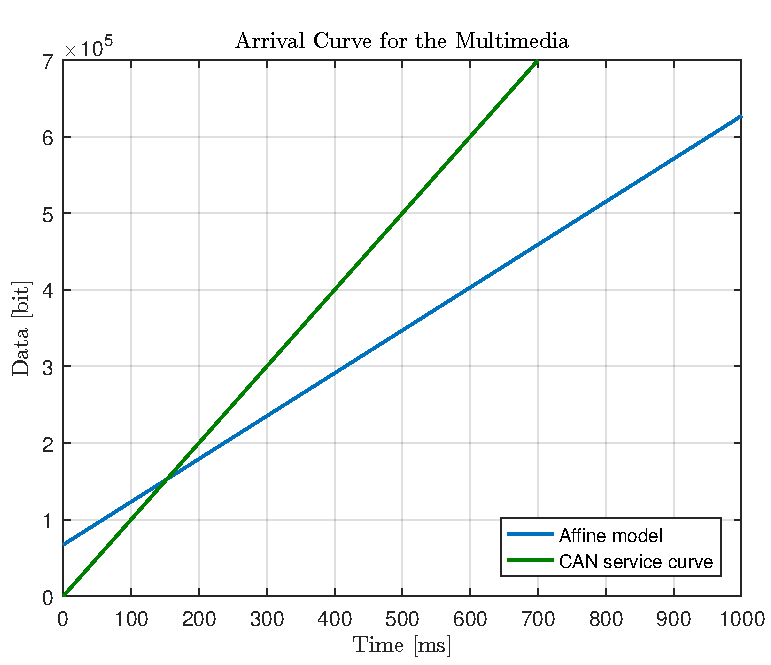
\includegraphics[width=.4\textwidth]{figures/ArrivalCurvesMultimedia}
	}
	\hspace{5pt}
	\captionbox
	{
		Arrival curves for the RC and service curve for the CAN-bus.
		\label{fig:ArrivalCurvesRC}
	}
	{
		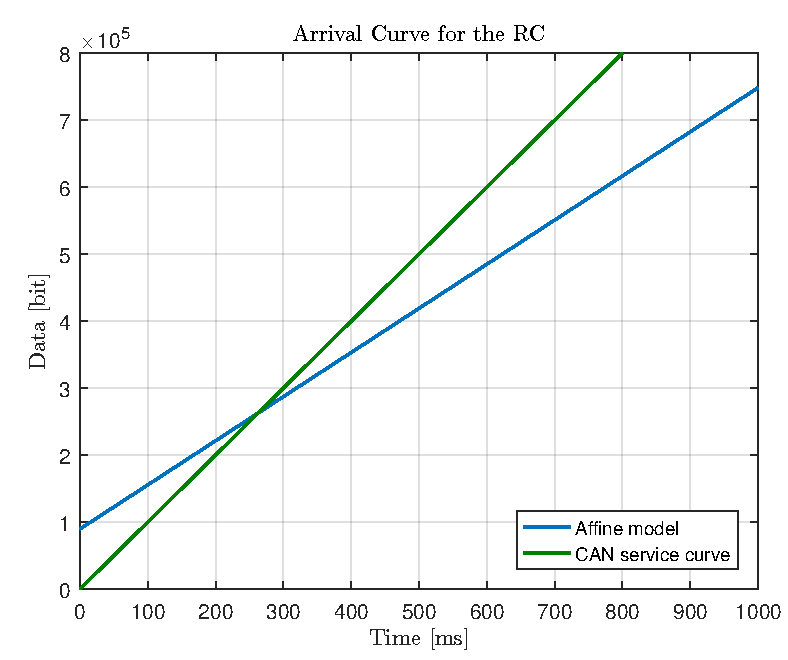
\includegraphics[width=.4\textwidth]{figures/ArrivalCurvesRC}
	}
\end{figure}
The maximum backlogs are given by the maximum vertical distance between the affine and the service curves before they cross, while the maximum waiting times by the maximum horizontal distance between the curves.
%
\begin{flalign}
    \mathrm{max\ backlog\ for\ the\ multimedia}&=67200\ \mathrm{bits}\nonumber \\
    \mathrm{max\ waiting\ for\ the\ multimedia}&=0.0672\ \mathrm{s} \nonumber\\
    \mathrm{max\ backlog\ for \ the\ RC}&=89600\ \mathrm{bits}\nonumber \\
    \mathrm{max\ waiting\  for \ the\ RC}&=0.0896\ \mathrm{s}\nonumber
\end{flalign}
